\section{Detecci\'on de ca\'idas}

Para poder detectar una posible caída del robot se cuenta con el giroscopio Gyro, incluido en el kit Bioloid de Robotis. Este giroscopio brinda información sobre la velocidad angular en los ejes $X$ y $Y$ como se muestra en la figura ~\ref{fig:gyroDireccion}.

\begin{figure}[hbtp]
\centering
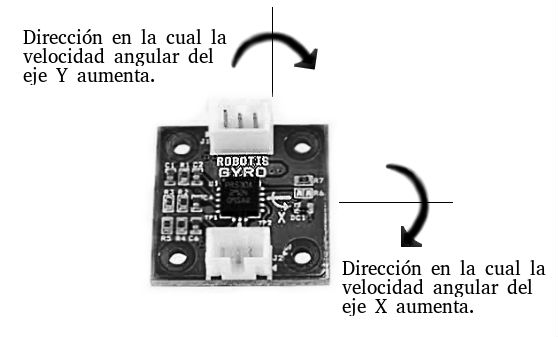
\includegraphics[scale=0.5]{imagenes/gyroDireccion.jpg}
\caption{Dirección en la que la velocidad angular de los ejes $X$ y $Y$, del Gyro, aumenta.}
\label{fig:gyroDireccion}
\end{figure}

La información del eje utilizado en este proyecto es el $X$, que indica si el robot experimenta una velocidad angular hacia adelante o hacia atrás. En la figura ~\ref{fig:gyroDireccion1} se muestra la direcci\'on en la que crece la velocidad angular con respecto al robot. El giroscopio puede detectar la velocidad desde $-300^{\circ}/s$ hasta $300^{\circ} /s$. Según la documentación, los valores que se leen del Gyro se dan en un rango de 45 a 445, en donde el valor 45 representa los $-300^{\circ}/s$ y el 455 representa los $300^{\circ} /s$. El valor 250 indica que no hay movimiento angular, es decir $0^{\circ}/s$. %Conociendo esta información, se decidió graficar los valores leídos por el giroscopio para observar su comportamiento mientras el robot ejecutaba una serie de movimientos.

\begin{figure}[hbtp]
\centering
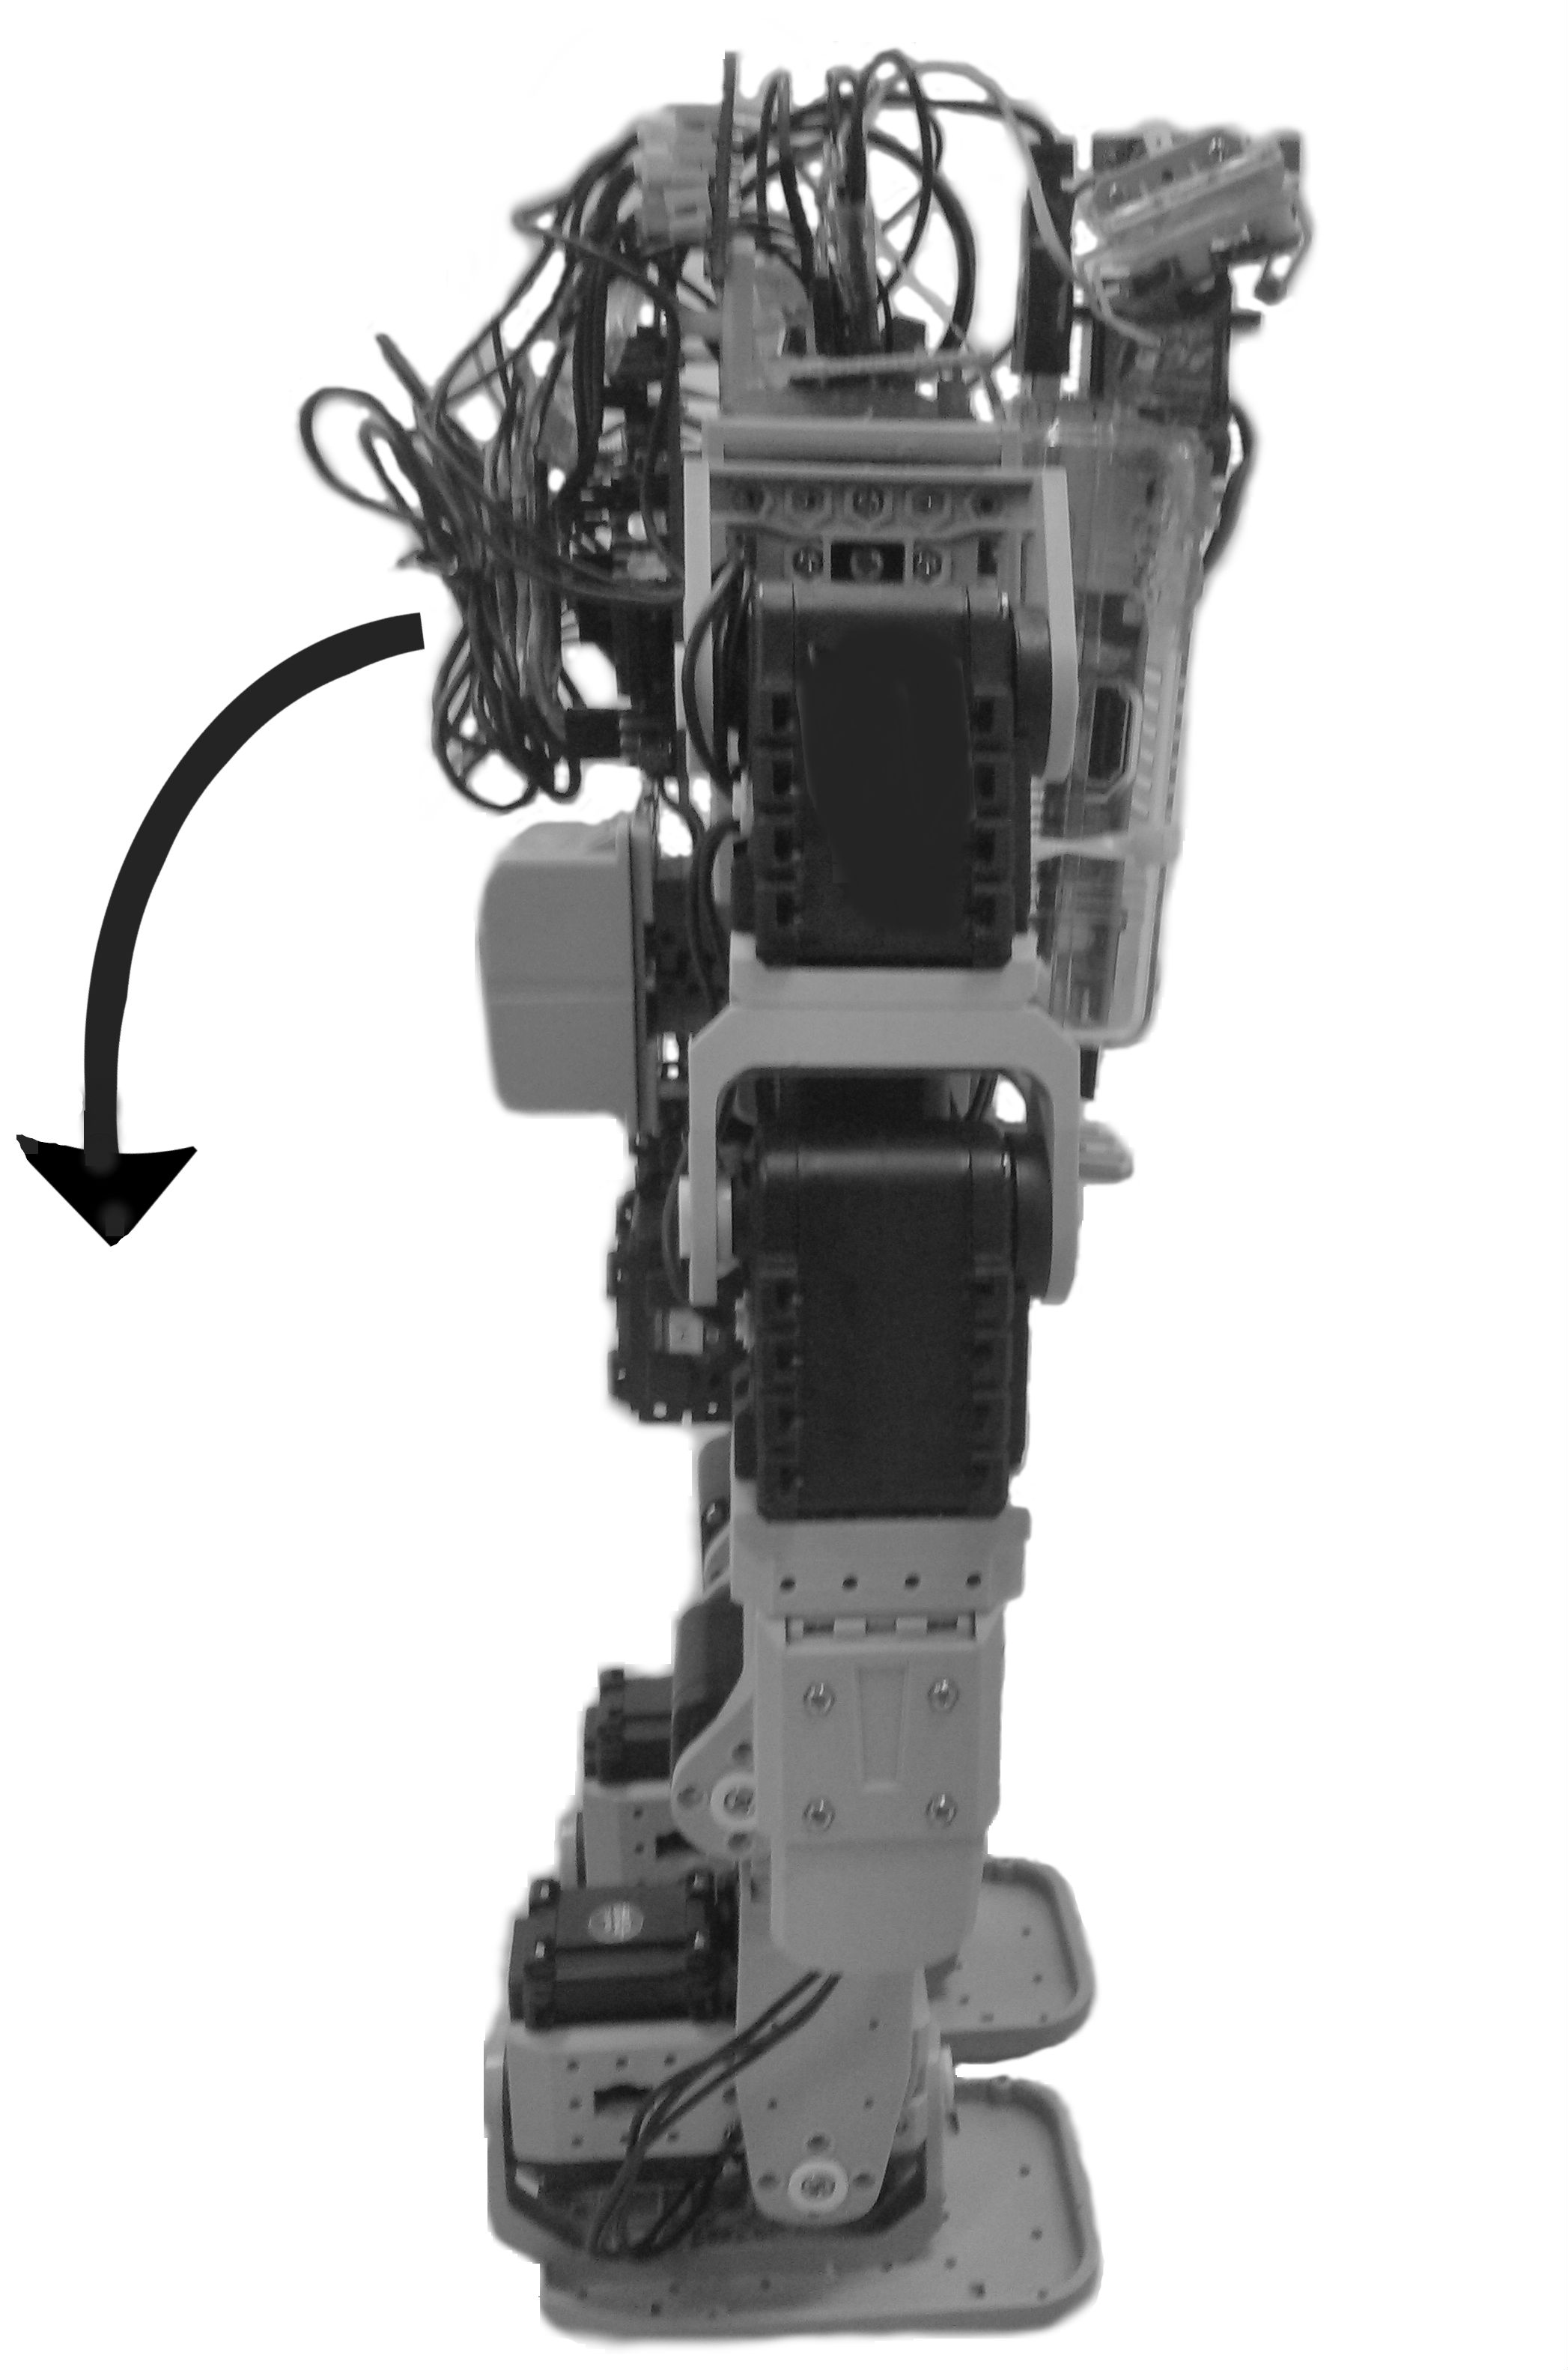
\includegraphics[scale=0.06]{imagenes/robotLateral.jpg}
\caption{Dirección en la que la velocidad angular del eje $X$ crece con respecto al robot.}
\label{fig:gyroDireccion1}
\end{figure}

%Se ha graficado los valores del giroscopio con el robot estático para comprobar que los valores leídos se corresponden con los de la documentación, es decir 250 cuando no hay movimiento. Cada punto representa un valor promediado de diez lecturas. La gráfica resultante es la que se puede apreciar en la figura ~\ref{fig:grafica1}. El primer valor promediado es 284 mientras que el último es 260. Por este motivo se decidió agregar un tiempo de 15 segundos del robot en reposo antes de comenzar la búsqueda de la pelota, de esta manera los valores del giroscopio se estabilizan. 

Para detectar una posible caída ha sido necesario verificar constantemente la velocidad angular del eje X. Se ha establecido un límite inferior y uno superior para identificar dentro de qué valores puede estar la velocidad angular sin que se considere como una caída del robot, sino como efecto de su movimiento. En caso de estar fuera de los límites, se considera como una caída y el robot ejecuta la acción de movimiento para levantarse.  

Se han observado los valores del giroscopio con el robot estático para verificar si los valores leídos se corresponden con los de la documentación, es decir 250 cuando no hay movimiento. Para obtener información más confiable se realiza un promedio entre diez lecturas para cada valor que se toma en cuenta. El resultado ha sido que los primeros valores no inician en 250 sino, en aproximadamente 284 y luego va disminuyendo. Por este motivo se decidió agregar un tiempo de 15 segundos del robot en reposo antes de comenzar la búsqueda de la pelota, de esta manera los valores del giroscopio se estabilizan. 

%\begin{figure}[hbtp]
%\centering
%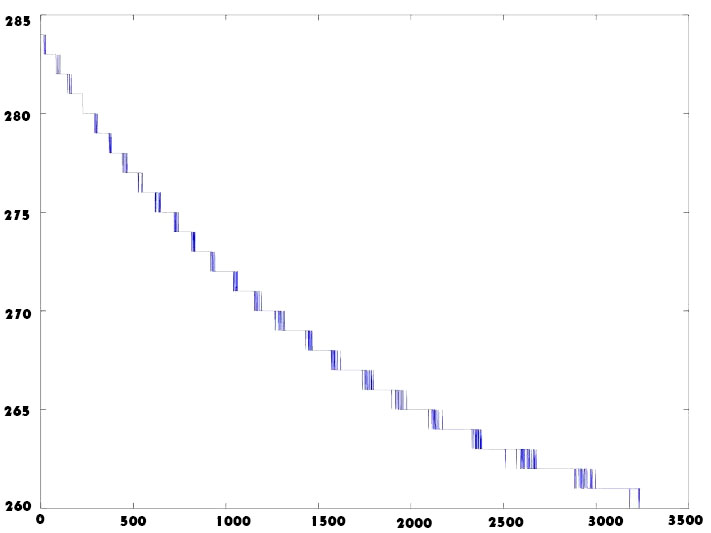
\includegraphics[scale=0.4]{imagenes/grafica1.jpg}
%\caption{Gráfica de lecturas de velocidad angular en el eje X.}
%\label{fig:grafica1}
%\end{figure}

Después de la pausa de 15 segundos, el primer valor promediado se toma como el valor que representa la velocidad angular cero, a este se le llamará valor central.   

%Una de las primeras gráficas se muestra en la figura X. Cada valor gráficado representa una lectura promediada de diez veces, mientras el robot ejecuta el movimiento de caminar repetidas veces. Se puede observar que los primeros valores se encuentran entre 300 y 350, luego los valores disminuyen en conjunto.   